\subsection{Mobiler \emph{Client}}

Beim RPISEC-Client handelt es sich um eine native Android App. Diese kommuniziert über REST-Schnittstellen mit einem OAuth-Server sowie mit Firebase-Diensten von Google. Die für diese App verwendeten Firebase-Dienste sind Firebase-Messaging und Firebase-RealTimeDatabase.\\

\subsubsection{Login}

Die Startseite der App besteht nur aus einem Login-Fenster (\autoref{fig:android_login}). Der Login erfolgt in zwei Schritten.

\begin{enumerate}
	\item OAuth Login\\
	\newline
	Die App generiert einen UUID-Wert (Universally Unique Identifier) als Identifikator für das Gerät. Zusammen mit dem eingegebenen Benutzernamen, Passwort und der UUID wird eine Anfrage für einen OAuth-Token an den OAuth-Server gestellt. Sind die Zugangsdaten korrekt, wird für diese UUID ein Token, sowie Client-Id und Client-Secret erzeugt und als Antwort an die App übertragen. Der OAuth-Token wird für die Authentifizierung bei den verbunden Diensten benutzt.\\
	
	\begin{code}
		\caption{ClientLoginOAuthTask.java}
		\yamlFile{\srcDir/ClientLoginOAuthTask.java}
		\label{src:ClientLoginOAuthTask}
	\end{code}
	
	\pagebreak
	
	\item  Firebase Login\\
	\newline
	Im zweiten Schritt wird ein Token für Firebase-Messaging registriert. Dies erfolgt wiederum mit dem Benutzernamen und Passwort. Nach der Registrierung kann die App Nachrichten über den Firebase-Messageing Dienst empfangen.\\
	
	\begin{code}
		\caption{RegisterFCMTask.java}
		\yamlFile{\srcDir/RegisterFCMTask.java}
		\label{src:RegisterFCMTask}
	\end{code}
\end{enumerate}

\begin{figure}[h]
	\centering
	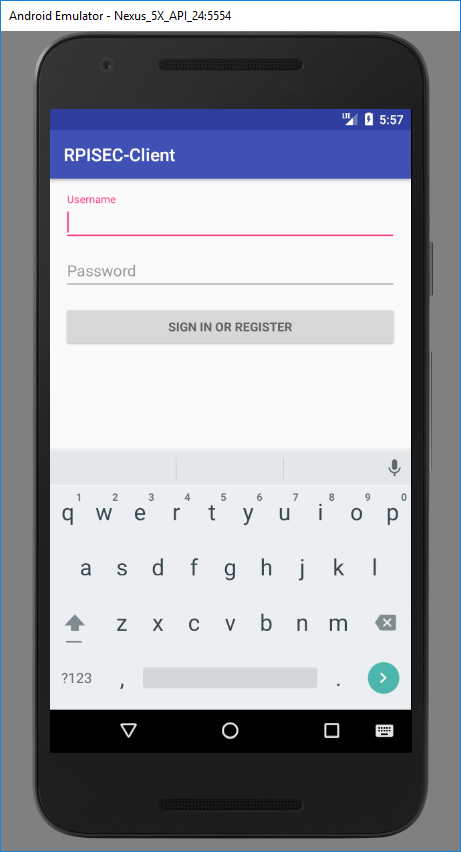
\includegraphics[scale=0.5]{\imageDir/android_login.png}
	\caption{Pin-Schema}
	\label{fig:android_login}
\end{figure}

Nach einem erfolgreichen Login wird automatisch die Detailansicht (siehe \autoref{fig:android_image_overview_m}) gestartet.

\pagebreak

\subsubsection{Detailansicht}

Bei der Detailansicht handelt es sich um eine Übersicht aller Bilder, chronologisch geordnet nach Aufnahmedatum, in einem Raster. Bei den angezeigten Bildern handelt es sich nur um Thumbnails. Die richtigen Bilder werden beim Auswählen eines Bildes angezeigt, ähnlich dem Fotoviewer in Android.\\

Die Detailansicht wird beim Eintreffen eines neuen Bildes aktualisiert. Sollte die Detailansicht nicht die aktive Anwendung sein, wird in der Infoleiste eine Notifikation angezeigt und ein Ton abgespielt. Durch tippen auf die Notifikation wird die Anwendung wieder in den Vordergrund geholt.\\

Mittels Swipe-Down-Geste kann die Ansicht aktualisiert werden.

\begin{figure}[h]
	\centering
	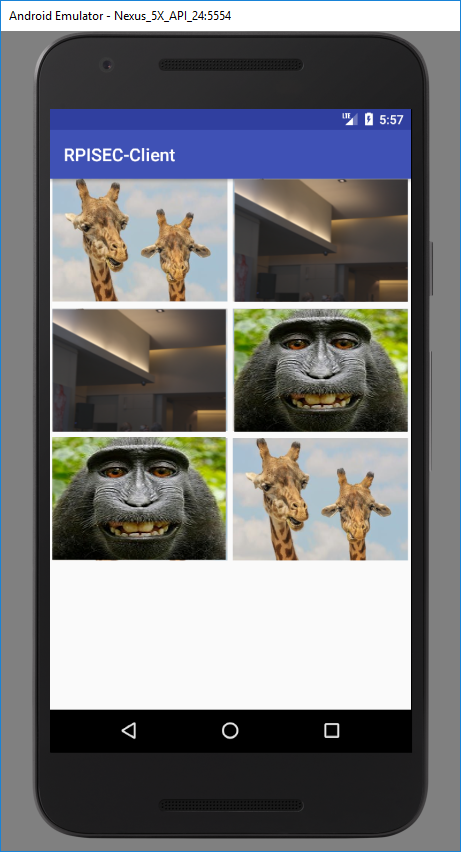
\includegraphics[scale=0.7]{\imageDir/android_image_overview_m.png}
	\caption{Pin-Schema}
	\label{fig:android_image_overview_m}
\end{figure}

\subsubsection{Datenabfrage}

Bei jedem \emph{Incident} der von der Server-Anwendung über Firebase-Messaging an die App gesendet wird, werden der Titel, eine Nachricht und die Id des aufgenommenen Bildes übertragen. Mit dieser Id kann das eigentliche Bild aus der Firebase-RealTimeDatabase abgerufen werden.\\

\begin{code}
	\caption{FirebaseMessaging.java}
	\yamlFile{\srcDir/FirebaseMessaging.java}
	\label{src:FirebaseMessaging}
\end{code}